\documentclass[12pt, a4paper]{report}

\usepackage[utf8]{inputenc}
\usepackage[T1]{fontenc}
\usepackage{lmodern}
\usepackage{graphicx}
\usepackage{amsmath, amssymb}
\usepackage{geometry}
\usepackage{setspace}
\usepackage{hyperref}
\usepackage[numbers]{natbib}  % For numeric citation style with natbib
\usepackage{listings}  % for code formatting
\usepackage{xcolor}  % For custom colors

% Page margins
\geometry{
    top=1in,
    bottom=1in,
    left=1.5in,
    right=1in
}

% Line spacing
\onehalfspacing
\lstset{
    language=Python,
    basicstyle=\ttfamily\small,      % Monospaced font
    keywordstyle=\color{blue},       % Reserved keywords in blue
    commentstyle=\color{green},      % Comments in green
    stringstyle=\color{red},         % Strings in red
    numbers=none,                    % Remove line numbers
    frame=single,                    % Add frame around the code
    breaklines=true,                 % Break long lines
    tabsize=4,                       % Tab size
    showstringspaces=false,          % Do not show underscores for spaces
    aboveskip=0pt,                   % Remove space above the code block
    belowskip=0pt,                   % Remove space below the code block
    lineskip=-1pt,                   % Reduce space between lines
    morekeywords={[1]self},
    morekeywords={[2]int, float, bool, tuple, list, Dataset, File, FemnistWriterDataset, HarDataset, torch, CnnEmnist, nn, Module, MaxPool2d, Conv2d, Linear, F, HarModel, ClientVerticalModel, ServerVerticalModel, FullVerticalModel},  % Type keywords
    keywordstyle=[2]\color{cyan},    % Type keywords in cyan
}

\begin{document}

\title{FL Studio - Uno Studio di Federated Learning}
\author{Daniele Tarek Iaisy}
\date{Ottobre 2024}
\maketitle

% Abstract
\begin{abstract}
Il federated learning è emerso come un promettente modello distribuito 
che permette ad un ampio numero di client di partecipare collettivamente
al training di un modello di machine learning, senza compromettere la 
privacy dei dati usati per il training, mantenendoli al sicuro alla 
fonte. Questo è un modello diametralmente opposto a quello del machine 
learning tradizionale in cui viene curato un unico dataset globale 
in cui vengono raccolti tutti i dati. Questa tesi si pone di studiare 
empiricamente come diversi gradi di ibridazione di approccio da quello 
completamente federato a quello completamente centralizzato influiscono
sulle performance del modello allenato.
Lo studio è stato condotto su due dataset di benchmark, il FEMNIST e 
l'UCI Human Activity Recognition (HAR) e permettendo di analizzare sia 
una CNN (Convolutional Neural Network) e una MLP (Multi Layer Perceptron)
entrambe di dimensioni contenute. 
Sono state provate diverse combinazioni
di percentuali di condivisione dei dataset (da 0\%, setting completamente
federato al 100\%, setting completamente centralizzato), di strategie 
di condivisione dei dati (scegliendo alcuni client di cui rendere i 
dataset condivisi o prendendo alcuni elementi dai dataset di tutti i 
client) e di diversi algoritmi di ottimizzazione.
I risultati sperimentali verificano che alte performance sono raggiungibili
anche in contesti completamente federati, anche se al costo di un 
maggiore numero di cicli di training.
\end{abstract}


\tableofcontents

\chapter{Introduzione}
La rapida proliferazione di dispositivi connessi sulla rete, insieme 
ad una maggiore sensibilità diffusa nei confronti della privacy 
hanno fatto sì che si rendessero necessari nuovi modelli di machine 
learning che tenessero in considerazione i requisiti di contesti 
privacy oriented. Il Federated learning (FL) è nuovo approccio che 
risolve questo problema permettendo a diversi client (ad esempio
telefoni, dispositivi IoT o server edge) distribuiti per il mondo di 
allenare collaborativamente uno stesso modello di machine learning. La 
privacy dei dati è preservata mantenendo i dati all'origine, sui 
client stessi che li producono, e portando invece il modello da 
allenare ad essi.

Nonostante le sue potenzialità, il federated learning ha comunque delle
difficoltà, prima fra tutte il fatto che tipicamente i dati locali 
dei client sono estremamente eterogenei tra loro, peggiorando le 
performance del modello allenato. Una delle assunzioni tipiche per le 
tecniche dei machine learning più diffuse è che il dataset utilizzato 
per l'apprendimento sia costituito da sample IID (Indipendenti e 
Identicamente Distribuiti), fatto che tipicamente non si verifica in 
contesti federati.

Una delle possibili strategie per migliorare le capacità di un modello 
allenato in modo federato è quella di costruire un dataset globale, 
composto da un sottoinsieme dei dataset dei client che viene condiviso 
e reso pubblico, il federated learning ibrido. Questa tesi studia la 
variazione di performance di un modello sotto diversi gradi di 
ibridazione. Vengono presi in considerazione due dataset diversi nel 
dominio dell'image classification e del human activity recognition 
-FEMNIST e UCI HAR- per vedere come si comporta il federated 
learning sotto diverse modalità. Il FEMNIST (Federated Extended MNIST)
è un'estensione del celebre MNIST che include immagini sia di cifre 
che di numeri e i cui caratteri sono partizionati in base allo scrittore
originale; l'UCI HAR invece contiene misurazioni fatte 
da accellerometro e giroscopio di uno smartphone tenuto in vita da 30
persone diverse mentre compiono azioni diverse. Per studiare al meglio 
gli effetti di diverse strategie di condivisione dei dati, si è 
allenata la stessa rete neurale con diversi gradi di condisione dei 
dati (da 0\%, federato, a 100\%, centralizzato) e diversi metodi di 
condivisione dei dati. Per il FEMNIST è stata usata una CNN e per UCI 
HAR un MLP. Entrambi i modelli sono stati allenati sia con SGD che 
con AdamW, due algoritmi di ottimizzazione tipici nel Deep Learning.


Questo elaborato è strutturato nel modo seguente: il capitolo 2 
introduce il federated learning, diverse categorizzazioni e strategie, 
seguiti da una discussione di vantaggi e limitazioni; il capitolo 3 
discute nel dettaglio gli esperimenti, descrivendo i dataset e i 
modelli usati e spiegando le scelte fatte; il capitolo 4 illustra 
l'implementazione del progetto in codice python, facendo uso di Flower
~\cite{flowerai}, un framework per fare simulazioni o applicazioni
di federated learning che supporta 
sia PyTorch che Tensorflow e vari ambienti di 
sviluppo oltre python tra cui Android, iOS e C++; infine il capitolo 5
mostra i risultati degli esperimenti e discute anche possibili metodi 
per migliorare ulteriormente le performance del modello.

\chapter{Federated Learning}
In questa sezione viene introdotto il Federated Learning, come funziona,
i diversi possibili approcci, quali sono i vantaggi e gli svantaggi.
Prima di tutto viene spiegato cos'è il Federated Learning e i diversi tipi
di partizionamento dei dati, mentre nel secondo paragrafo vengono discussi
gli aspetti positivi di questa tecnica, specie nell'area della privacy dei
dei dati per contesti ad alta sensibilità. Infine vengono discusse le
difficoltà che quest'approccio provoca, principalmente la distribuzione non
IID (Indipendent and Identically Distributed) dei dataset locali.

\section{Come funziona}
Il Machine Learning è la classe di algoritmi di apprendimento in cui ad un
modello viene fornito un insieme di dati, il training dataset, da cui
imparare una certa funzione obbiettivo su questi dati. Un algoritmo di 
Machine Learning popolare una decina di anni fa era quello delle SVM
(Support Vector Machine), mentre ad oggi il Deep Learning la fa da padrona.
Tipicamente, nei problemi di Machine Learning si assume di avere un unico
dataset e un unico modello che ha accesso a tutti i sample nel dataset.
Tuttavia quest'approccio può porre alcuni problemi: in contesti in cui si
lavora con dati sensibili, come i dati medici di privati cittadini, può 
essere sconsigliato, difficile o vietato (da norme come il GDPR o il più
recente AI act) raccogliere tali dati da utilizzare per allenare un modello;
inoltre la creazione e gestione di un tale dataset può avere costi non
indifferenti dati dal trasporto dei dati in unico data storage centralizzato,
la memorizzazione di tali dati e il costo dell'effettivo allenamento del
modello.

Il Federated Learning si pone di risolvere questo problema allenando il nostro
modello proprio alla fonte dei dati, dove questi sono già presenti o vengono
generati. In questo framework possiamo individuare N client ognuno dei quali
ha una copia del modello da allenare fornitagli da un server e ognuno dei quali
con il proprio dataset, disgiunto da quello degli altri client.
Ad ogni round di apprendimento ognuno degli N client allena il proprio modello 
con il proprio dataset locale e, finito il passo di apprendimento, invia al
server il proprio modello aggiornato. A questo punto il server si occuperà 
semplicemente di fare una qualche aggregazione dei nuovi N modelli che gli sono
stati forniti e redistribuire ai client il nuovo modello prodotto.

In questo studio ci occupiamo di applicare il Federated Learning a 2 reti neurali,
un semplice MLP (Multi Layer Perceptron) e una CNN (Convolutional Neural Network),
ma questa tecnica può essere usata in tutti gli algoritmi di Machine Learning in 
cui modello usato permette un qualche meccanismo di aggregazione; le reti neurali
non sono uniche in questo e le già citate SVM sono un altro di questi casi.

A seconda di come differiscono i dataset locali di ogni client si possono
fare 2 classificazioni di Federated Learning: quello a partizionamento orizzontale
e quello a partizionamento verticale.

\section{Metodi di partizionamento}
Uno dei punti fondamentali del federated learning è come sono 
distribuiti i dati tra i vari client. Si possono individuare almeno due 
categorie di federated learning in base a come sono distribuiti: 
l'Horizontal Federated Learning (HFL) e il Vertical Federated Learning
(VFL). In questa sezione vengono presentati i due modelli e poi vengono 
anche discusso un modello ibrido in cui parte dei dati rimane alla fonte 
e un'altra parte viene condivisa in un unico dataset globale.

\subsection{Partizionamento orizzontale}
Nel partizionamento orizzontale, detto anche sample-based federated 
learning, i dataset di tutti i client hanno lo
stesso schema, le stesse features, e i dataset variano per i sample
che contengono. Un esempio di questo caso, con cui tutti abbiamo a che 
fare ogni giorno, sono i suggeritori di testo nelle tastiere dei 
nostri smartphone, in cui ogni telefono ha la copia di uno stesso 
modello di partenza e le feature di input a questo modello sono sempre 
le stesse, una stringa che abbiamo scritto noi, ma i dataset locali 
di ogni telefono sono diversi perché includono solo i messaggi scritti 
su quel telefono. In questo modo si ottiene la personalizzazione del 
suggerimento di testo.


\subsection{Partizionamento verticale}
Nel partizionamento verticale VFL, conosciuto anche come feature-based 
federated learning, ogni client utilizza un insieme 
di feature diverse da quelle degli altri, con un qualche collegamento 
tra i sample. Un primo studio che ha introdotto il VFL in modo distinto
da quello orizzontale è yang et al. ~\cite{yang2019vfl}.
In questo caso i dati non vengono da una 
fonte comune istanziata più volte (come la stessa applicazione che 
produce gli stessi dati usata da utenti diversi), ma fonti diverse,
eterogenee e tipicamente indipendenti tra loro, che seppur essendo
dati diversi fanno riferimento alla stessa "entità" (come ad esempio
una persona). Un esempio concreto di questa situazione può essere 
quello di una banca e una società di e-commerce che hanno informazioni
diverse sugli stessi clienti. L'obbiettivo del VFL in questo caso è
quello di allenare un modello globale che possa predire o analizzare
il comportamento dei clienti, evitando di dover condividere le loro 
informazioni tra la banca e la società di e-commerce.
Per fare ciò, ogni parte coinvolta avrà un proprio modello locale che 
calcola un embedding delle feature. Questi embeddings vengono poi
raccolti e forniti ad un modello globale che finisce di calcolare la 
funzione obbiettivo.

Una delle principali difficoltà del VFL, assente nel HFL, è quella 
di allineare le diverse feature tra le varie organizzazioni, in 
modo che però non avvenga uno scambio di esse. Un altro problema è 
quello dello scambio degli embeddings in modo sicuro senza che da 
questi si riesca a risalire alle feature originali, invertendo
l'operazione di embedding. Questo tipo di problemi in genere può 
essere risolto facendo uso di Differential Privacy (DF) e/o di 
homomorphic encryption; alcuni studio che discutono questi problemi e
come risolverli sono Wei et al. ~\cite{wei2022vflChallenge} e 
~\cite{liu2022vflChallenge}


\subsection{Ibridazione}
In contesti in cui la privacy non è un requisito fondamentale, dove il
federated learning può essere applicato per distribuire i calcoli e 
ottenere personalizzazione sui dati piuttosto che garantire la privacy
degli utenti, un'idea interessante è quella seguire un approccio ibrido 
tra quello del federated learning e il machine learning tradizionale.
L'idea è quella di condividere solo una piccola percentuale di dati 
in modo da migliorare le performance del modello, pur mantenendo lo 
spostamento di dati al minimo. Quest'interesse è motivato da risultati 
empirici come quelli di Zhao et al. ~\cite{zhao2018flniid} che hanno 
visto come condividendo solo il 5\% dei dati si può ottenere un 
miglioramento del 30\% sulla precisione del modello.

Se ci si pone in un contesto di federated learning ibrido, anche qua,
possiamo avere diversi modelli di condivisione dei dati. Un approccio 
può essere quello di una condivisione client-based in cui alcuni client 
condividono interamente i loro dataset. La selezione dei client può 
essere fatta sia in modo centralizzato, dallo stesso server che gestisce 
il modello globale, che su base volontaria in cui un utente può decidere 
spontaneamente di condividere i propri dati.
Un'altra alternativa può essere quella di stabilire un certo quantitativo,
come una percentuale fissata o un numero costante di sample, che ogni 
client deve contribuire al dataset globale, mantenendo il resto dei 
propri dati privati.


\section{Strategie di aggregazione}
Nel federated learning un punto importante è la strategia di aggregazione
usata per aggiornare il modello globale una volta ricevuti gli update 
dei modelli dei client. In questa sezione viene prima di tutto introdotta 
la \textit{FedAvg} la prima e più famosa strategia. Notati i problemi 
di questa strategia, vengono poi discusse altre strategie presenti 
nella letteratura che puntano a migliorarne i punti deboli, come 

\subsection{FedAvg}
La strategia più conosciuta ed usata è la \textit{FedAvg} (Federated
Averagin), introdotta in McMahan et al. ~\cite{McMahan2016CommunicationEfficientLO},
paper che introduce per la prima volta il federated learning. Nel 
\textit{FedAvg} il server aggrega i nuovi parametri calcolando una 
media pesata di tutti quelli ricevuti, dove il peso dato ad ogni modello
è la dimensione del dataset locale usato rapporta al numero totale di 
sample usati nel round di training. In pratica, dati \(K\) client,
ognuno con la propria copia \(\theta_t\) dei parametri del modello globale 
al round \(t\) e con il proprio dataset locale di dimensione 
\(d^k\), per \(k = 1, \dots, K\), denotando con 
\(D := \sum_{k=1}^{K} d^k\), il numero totale di sample usati in
questo round di training, i parametri del modello globale al round 
\(t+1\) sono calcolati con 
\[
\theta_{t+1} := \sum_{k=1}^{K} \frac{d^k}{D} \theta_t^k
\]

Questa è una tecnica semplice da capire e da implementare, ottima per 
eperimenti di benchmark e feasibility studies ed è la strategia 
utilizzata anche per questo studio. Tuttavia, è una strategia che 
assenga ad ogni sample di ogni dataset lo stesso peso relativo sul 
risultato del modello globale e ciò fa si che \textit{FedAvg} possa 
fare fatica in contesti molto non-IID.


\subsection{FedProx}
Riconoscendo il problema dell'eterogeneità dei dati e delle capacità 
computazionali di client diversi, Li et al. ~\cite{li2018FederatedOI}
introducono una nuova strategia di aggregazione chiamata 
\textit{FedProx}. Tale strategia funziona in modo analogo a 
\textit{FedAvg} con la sola differenza che ogni client \(k\), anziché 
minimizzare la propria normale loss function \(L^k\), minimizza la 
funzione
\[
L^k(\theta^k) + \frac{\mu}{2} ||\theta^k - \theta_t||^2
\]
dove il termine di prossimità \(\frac{\mu}{2} ||\theta^k - \theta_t||^2\) 
penalizza l'allontanarsi molto dal modello globale corrente
\(\theta_t\) analogamente a come funziona la regolarizzazione \(L_2\),
introducendo l'iperparametro \(\mu\).

Oltre a ridurre l'impatto che l'eterogeneità che ha i dataset locali 
sulle performance del modello globale, facendo si che i modelli locali 
non possano allontanarsi eccessivamente da quello globale, permette 
anche un maggiore grado di eterogeneità delle prestazioni computazionali 
dei client. Se con la \texit{FedAvg}, infatti, client che compiono 
molte epoche di apprendimento velocemente rischiano ritrovarsi con un 
modello significativamente diverso da uno di un client che ha compiuto
pochi cicli di allenamento, forzando quindi round di sincronizzazione
che hanno l'effetto di far andare l'intera rete alla velocità del più
lento o scartando interamente i nodi più lenti dal sistema federato, 
il fatto di non potersi allontanare troppo dal modello globale fa si
che sia più difficile che modelli locali possano divergere tra loro,
rendendo l'intero sistema più efficiente e stabile.


\subsection{SCAFFOLD}
SCAFFOLD (Stocastic Controlled Averaging for Federated Learning) è una 
strategia introdotta in ~\cite{Karimireddy2020scaffold} per 
affrontare il problema del client drift, ovvero quella situazione in 
cui i modelli locali tendono a divergere gli uni dagli altri e allontanarsi 
da un minimo globale, producendo overfitting sui loro dataset locali 
e rallentando la convergenza del modello globale.
In questa strategia viene introdotto il concetto di control variate
\(c\), ovvero un ulteriore tensore con la stessa dimensione del modello 
che sta venendo allenato, utilizzato per ridurre il client drift. 
Esiste un control variate globale \(c_t\) ed uno locale \(c_t^k\) per 
ogni client. Ogni client calcola l'aggiornamento dei suoi parametri come:
\[
\Delta\theta_{t+1}^k = \eta (\nabla L^k(\theta_t^k) -c_t^k +c_t)
\]
dove \(\eta\) è il learning rate e \(L^k\) è la loss function del 
client \(k\). Dopodiché il server aggiornerà il modello globale con:
\[
\theta_{t+1} = \theta_t + \frac{1}{K} \sum_{k=1}{K} \Delta\theta_{t+1}^k
\]

\subsection{Summary}
Come spesso accade non esiste una \textit{one size fits all} e diverse 
strategie hanno diversi pro e contro. Inoltre la necessità o efficiacia 
di strategie diverse dipende significativamente dai dati e le prestazioni 
dei client dello specifico sistema. Si possono però tracciare delle 
linee generali analizzando le performance di diverse strategie sugli 
stessi dataset di benchmark. Esistono infatti diversi studi comparativi 
di diverse strategie come Kairouz et al.  ~\cite{kairouz2021flOpenProblems}.


\section{Vantaggi}
Il federated learning offre vantaggi significativi sia in termini di 
privacy che in termini di costo di infrastruttura. 
Uno dei primi  vantaggi è la possibilità poter allenare un modello 
di machine learning in modo distribuito, potendo scaricare parte del 
\textit{compute} sull'edge anziché sull'organizzazione che fornisce 
il modello, fattore interessante se si considerano i costi elevati che 
si incorrono nell'allenare modelli allo stato dell'arte.
Inoltre in questo setting non c'è bisogno di inviare i dati in unica 
repository centralizzata, potendo quindi preservare la privacy degli
utenti che generano tali dati, eliminando la necessità di 
un'infrastruttura di database o datawarehouse per l'ente che gestisce
il modello ed eliminando il carico sulla rete per trasmettere tali
dati, fattori che possono diventare significativi se se il learning è
fatto su larga scala come ad esempio sulla miriade di dispositivi IoT.

\section{Problemi}
Nonostante i suoi vantaggi, il federated learning presenta anche delle 
difficoltà.
In primis, c'è il fatto che dato che i dati locali sono tipicamente 
eterogenei e dotati di bias. In particolare non sono IID (Independent
and identically distributed), condizione spesso richiesta nel 
machine learning. Il risultato è che ogni client quando allena modello 
gli insegna lo stesso bias presente nel suo dataset. Particolarmente
significativo è lo sbilanciamento delle classi in problemi di 
classificazione ~\cite{zhao2018flniid} ~\cite{xiao2021flci}.
Inoltre, pur non necessitando di dover inviare dati in ad al server è
ancora necessario inviargli i modelli aggiornati nel caso del 
partizionamento orizzontale o l'embedding delle feature nel caso 
verticale. Se i round di comunicazione tra client e server sono 
frequenti è possibile che questo risulti in un utlizzo di rente 
significativamente più alto, fattore che può essere problematico
specialmente per i client in caso abbiano risorse limitate come reti 
mobili per telefoni o dispositivi IoT, oltre che un elevato uso di 
energia che può rapidamente consumare le batterie.
Un altro problema significativo può essere quello di un leaking di 
dati sensibili attraverso un \textit{inference attack} a partire 
dai parametri aggiornati del modello o dal feature embedding. Questi 
problemi possono essere risolti con tecniche come la differential 
privacy o l'homomorphic encryption, ma questo comporta un costo 
computazionale maggiore dell'intero processo e può degradare ancora 
le performance del modello.
In utlimo, il federated learning rimane un modello di computazione 
distribuita e come tale pone tutte le difficoltà di comunicazione e 
sincronizzazione tipiche di quest'approccio.


\subsection{Sintesi}
Conclundendo, il federated learning è un approccio al machine 
learning che offre svariati vantaggi, dalla distribuzione del 
calcolo per l'allenamento, alla personalizzazione del comportamento 
del modello in funzione dell'utente, alla protezione della 
privacy dei dati in contesti di dati sensibili.

Tuttavia questi benefici si ottengono al costo di dover gestire
un sistema distribuito, invece di un unico server cloud, e 
soprattutto diventa una grande fonte di eterogeneità dei dati,
rendendoli non-IID e limitando le performance del modello 
allenato. Per tale motivo il federated learning rimane una 
tecnica potente ma da utilizzare con attenzione nei contesti 
in cui risulta utile o necessario, come ad esempio nel caso in 
cui esistano regolamentazioni a protezione dei dati.

\chapter{I Dataset}
In questa sezione vengono introdotti i dataset usati per i nostri
esperimenti. Il primo dei due è il FEMNIST, cioè l'EMNIST 
in cui ogni lettera o numero sono raggruppati in base alla 
persona che li ha scritti; il secondo è l'UCI HAR un dataset per il
riconoscimento dell'attività dell'utente in base a misurazioni fatte
da un dispositivo che ha addosso, come l'accellerometro di smartphones
o smart watches.

\section{FEMNIST}
Il famoso dataset MNIST (Modified National Institute of Standards and
Technology), l'Hello World del Machine Learning, nasce nel 1994 creato 
da LeCun et al.~\cite{lecun1998mnist} partendo dai un altro dataset 
del NIST.
Il MNIST è stato creato a partire dai dataset SD-1 e SD-3 (Special
Dataset). Lo SD-3 veniva usato come training set e conteneva immagini
di cifre scritte a mano da impiegati dell'American Census Bureau,
mentre lo SD-1, usato come test set, erano cifre scritte a mano da 
studenti delle scuole superiori americane. Le cifre degli studenti
erano però scritte con una calligrafia più difficile da leggere, rendendo più 
difficile trarre conclusioni sulle capacità del modello alla fine del
training. Per questo motivo è stato creato un unico dataset, l'MNIST 
che contiene un totale di 60'000 immagini di cifre sia degli studenti
che degli impiegati dell'American Census Bureau.

L'EMNIST (Extended MNIST) è un'estensione del dataset originale,
pubblicata nel 2017 da Cohen et al.~\cite{cohen2017emnist} nata 
per rendere il problema più difficile, viste le performance altissime
che le CNN ottengono con poche epoche di training sul MNIST originale.
Nasce dall'unione di altri dataset gestiti dal NIST, include cifre e
anche lettere sia maiuscole che minuscole, per un totale di 62 classi.
L'MNIST originale include cifre scritte da circa 250 persone diverse,
mentre l'EMNIST contiene dati da 3597 persone diverse e un totale di 
814'255 sample diversi.

Per finire, il FEMNIST (Federated EMINST)
viene introdotto in Caldas et al.~\cite{caldas2019femnist}
ed è un dataset che include tutti i sample dell'EMNIST partizionati
per scrittore originale, in modo da poter essere utilizzato in contesti
di apprendimento federato, in cui ogni client esegue il training non su
tutti i sample dell'EMNIST, ma solo quelli dello scrittore originale
corrispondente.

Come tutti i suoi predeccessori, il FEMNIST è un dataset che contiene
immagini di 28x28 pixel in greyscale, quindi ad un unico canale. Le
cifre e lettere sono tutte centrate nell'immagine in base centro di 
massa dei pixel del carattere.
Il dataset originale è stato costruito da, tra gli 
altri, dipendenti di google e come tale è stato pensato per funzionare
nativamente con Tensorflow. La repository originale per generare il
dataset può essere trovata su github ~\cite{leaf_repo}. Dato che però
il codice per questi esperimenti è stato scritto nel framework di PyTorch,
seguendo il dataset loader indicato su Papers with Code ~\cite{femnist_pwc},
per generare il dataset è stata usata la repository di Xiao Chenguang 
~\cite{femnist_hdf5}, che permette di generare un file \texttt{.hdf5} contenente
l'intero dataset, potendo anche scegliere se includere tutti i caratteri
o solo le cifre come nel MNIST originale. Quella che segue è la funzione
utilizzata per aprire il dataset \texttt{.hdf5} creato utilizzando questa repository
e istanziare i Dataset di PyTorch per ognuno dei client usati nella
simulazione:

\clearpage
\begin{lstlisting}
    def _get_femnist_datasets(
        num_writers: int,
        val_ratio: float,
        test_ratio: float,
        only_digits: bool = False,
    ) -> tuple[list[Dataset], list[Dataset], list[Dataset]]:    
        dataset_file = "write_digits.hdf5" if only_digits else "write_all.hdf5"
        full_dataset = h5py.File(f"data/{dataset_file}", "r")
        writers = sorted(full_dataset.keys())[:num_writers]
        train_sets = []
        val_sets = []
        test_sets = []
    
        for writer in writers:
            images = full_dataset[writer]["images"][:]
            labels = full_dataset[writer]["labels"][:]
            client_dataset = FemnistWriterDataset(
                images, labels, transform=femnist_transform
            )
    
            train_subset, val_subset, test_subset = _split_dataset(
                client_dataset, val_ratio, test_ratio
            )
            train_sets.append(train_subset)
            val_sets.append(val_subset)
            test_sets.append(test_subset)
    
        full_dataset.close()
        return train_sets, val_sets, test_sets
\end{lstlisting}

Tutti gli argomenti di questa funzione sono controllabili tramite la
configurazione Hydra usata per eseguire lo script. Si noti come
l'implementazione supporti anche un test di validazione per una 
possibile implementazione di early-stopping. I dataset di validazione 
sono però stati ignorati nel corso degli esperimenti.


\section{UCI HAR}
L'UCI HAR (University of California Irvine -
Human Activity Recognition) è un dataset diverso dal FEMNIST. In primis
non è un dataset di computer vision, ma di human activity recognition.
Il dataset è stato introdotto in ~\cite{Anguita2013APD} e la fonte dei
dati sono accellerometri e giroscopi di smartphones.

Negli esperimenti condotti 30 volontari di età compresa tra i 19 e i 48 anni
hanno compiuto diverse azioni avendo uno smartphone legato in vita 
usato per registrare l'accelerazione lineare e la velocità 
angolare 3-assiale. Lo smartphone usato è un Samsung Galaxy SII, le 
misurazioni sono state fatte ad una frequenza di 50Hz e le azioni compiute
sono il camminare, salire o scendere le scale, sedersi, alzarsi e 
sdraiarsi, per un totale di 6 classi di azioni diverse.
I sample del dataset non sono però sequenze di misurazioni; dopo 
aver misurato velocità e accelerazione, grandezze vettoriali 3-dimensionali,
e aver rimosso rumore dai segnali con un filtro Butterworth low-pass 
~\cite{butterworth_filter}, è stata fatta un'aggregazione di tutti i 
valori in una finestra temporale di 2.56s. Tale aggregazione produce 
561 valori reali che vengono organizzati in un unico feature vector 
che funziona da input del modello. La label è l'azione che stava venendo
compiuta in quei 2.56 secondi.
Scaricati i file del dataset, disponibile sul sito della 
University of California Irvine ~\cite{uci_har_ds}, sui file 
\texttt{README.txt} e \texttt{features\_info.txt}
si posso trovare informazioni dettagliate sul 
processing fatto per estrarre le 561 feature, mentre su youtube 
~\cite{har_measuring_video} è disponibile un video che mostra il 
processo di registrazione delle azioni.

Il dataset include un totale di 10299 vettori di feature che sono stati
già divisi randomicamente 
in un test set del 30\% del totale e in un training set 
che contiene il 70\% delle feature.
Quella che segue è la funzione utilizzata per aprire i file del 
dataset come sono forniti dall'UCI i Dataset di PyTorch per 
ognuno dei client 30 e partizionare correttamente i sample:

\clearpage
\begin{lstlisting}
def _load_har_dataset(train: bool):
    variant = "train" if train else "test"
    full_features = [[] for _ in range(30)]
    full_labels = [[] for _ in range(30)]

    # get subject ids for measurements
    with open(f"data/subject_{variant}.txt", "r") as subject_file:
        subject_ids = [int(line.strip()) - 1 for line in subject_file]
    # get features and match them with the user
    with open(f"data/X_{variant}.txt", "r") as feature_file:
        for i, line in enumerate(feature_file):
            features = [float(num) for num in line.split()]
            full_features[subject_ids[i]].append(features)
    # get labels and match them with the user
    with open(f"data/y_{variant}.txt", "r") as label_file:
        for i, line in enumerate(label_file):
            label = int(line)
            one_hot = torch.zeros(6, dtype=torch.float32)
            one_hot[label - 1] = label
            full_labels[subject_ids[i]].append(one_hot)

    if train:
        return full_features, full_labels
    # flatten in one dataset for testing
    else:
        return [
            feature for user_features in full_features for feature in user_features
        ], [label for user_labels in full_labels for label in user_labels]


def _get_har_datasets() -> tuple[list[Dataset], Dataset]:
    train_features, train_labels = _load_har_dataset(True)
    test_features, test_labels = _load_har_dataset(False)

    client_datasets = [
        HarDataset(
            features=torch.tensor(train_features[cid], dtype=torch.float32),
            labels=train_labels[cid],
        )
        for cid in range(len(train_features))
        # some clients dont include measurements in the trainset
        if len(train_features[cid]) > 0
    ]
    test_dataset = HarDataset(
        torch.tensor(test_features, dtype=torch.float32), test_labels
    )
    return client_datasets, test_dataset
\end{lstlisting}

In questo caso la logica per istanziare il dataset federato è stata 
divisa in due funzioni in quanto, diversamente dal FEMNIST in cui il 
dataset originale è già partizionato per client, in questo caso c'è 
bisogno di (i) aprire 3 file diversi \texttt{subject\_\{variant\}.txt}, 
\texttt{X\_\{variant\}.txt} e \texttt{y\_\{variant\}.txt} e riassociare 
i dati tra loro e (ii) instanziare i \texttt{Dataset} di PyTorch.
La funzione \texttt{\_load\_har\_dataset} si occupa di fare la prima tasks,
mentre \texttt{\_get\_har\_datasets} si occupa di istanziare correttamente le classi 
\texttt{Dataset}. Si noti che i dataset locali sono partrizionati per 
utente, mentre il dataset di test è un unico dataset con sample di 
tutti gli utenti.
\chapter{Implementazione}
In questo capitolo viene descritta l'implementazione degli esperimenti
e vengono discusse le scelte implementative.
La prima sezione è dedicata agli strumenti utilizzati. Per prima cosa
viene introdotto PyTorch, il framework usato per 
definire le reti neurali usate, dopo viene introdotto Flower un 
framework per implementare e simulare sistemi di federated learning.
Infine viene introdotto anche Hydra un framework per configurare 
molteplici esperimenti di datascience in python comodamente.

La seconda sezione invece è dedicata alle implementazioni fatte per 
questi esperimenti. In primis, vengono descritti i modelli usati per
i diversi. Successivamente viene discussa l'ibridazione implementata 
dal modello di 
apprendimento federato a quello centralizzato, condividendo acluni 
sample dei dataset dei client in un unico dataset centralizzato.


\section{Gli strumenti}
\subsection{PyTorch}
PyTorch ~\cite{pytorch} è una libreria open-source estremamente popolare e flessibile 
per programmare ed allenare modelli di Deep Learning.
Siluppata inizialmente dal FAIR lab (Facebook's AI Reasearch), offre
un'API dichiarativa in python per costruire architetture di reti 
neurali, lasciando totale controllo al programmatore sul passo di 
feed forward di dati, facilitando la rapida sperimentazione di 
approci diversi e l'implementazione di pipeline
complesse come le GAN (Generative Adversarial Nets) ~\cite{goodfellow2014gan},
sperimentare tra transformer encoder-decoder ~\cite{vaswani2017trans}
o decoder only ~\cite{Radford2018ImprovingLU}.

PyTorch include una libreria estensiva di diversi tipi di layer,
loss functions, funzioni di attivazione e algoritmi di ottimizzazione
e la feature di autograd,
per cui facendo uso di un grafo dinamico di computazione PyTorch 
gestisce in automatico il calcolo del gradiente della loss function 
rispetto ad ogni parametro, rende l'implementazione di reti neurali 
estremamente facile, specie per casi particolarmente complicati 
come CNNs o RNNs.

\subsection{FlowerAI}
Flower (o FlowerAI) ~\cite{flowerai} è un framework open-soruce progettato semplificare
l'implementazione di sistemi di federated learning. Pur essendo una 
libreria python, supporta anche SDK per Android, iOS e c++, rendendolo 
ideale anche in ambienti mobile o di IoT.
Flower fornisce un'API per definire e implementare comodamente ogni 
specifico client in un apprendimento federato, configurandone il modello
da allenare, l'algoritmo di training e valutazione. Allo stesso modo è 
controllabile il comportamento del server e la strategia di aggregazione 
dei parametri aggiornati del modello forniti dai client  (i.e. un oggetto
di tipo flwr.server.strategy.Strategy).

Flower è stato usato per eseguire le simulazioni di apprendimento 
federato sui dataset FEMNIST e UCI HAR. In ogni simulazione, ogni client 
ha allenato il suo modello locale per un numero basso di epoche (5 per 
l'UCI HAR, 6 per il FEMNIST) e dopodiché manda i parametri aggiornati 
al server. La strategia utilizzata per aggregare i server è la
FedAvg. Questo ciclo  di allenamento e aggregazione 
costituisce un round ed ogni simulazione 
è durata 20 round.

Va notato che Flower è un framework pensato principalmente per il 
federated learning orizzontale e non ha un supporto nativo per 
contesti a partizionamento verticale. La soluzione, suggerita dallo 
stesso team di Flower ~\cite{flower_vfl}, è quella di riutilizzare 
il meccanismo di scambio di parametri da client a server per passare
invece l'encoding delle feature calcolato dal modello locale. 
L'effetto collaterale di questo sistema è che l'intero feed forward 
delle feature, nei modelli locali dei client ad encodings e poi 
nel modello del server da encoding a classificazione, richiede l'intero 
round di training. Questo implica che ogni round può eseguire una sola
epoca di training per round, cosa che può essere aggirata moltiplicando
il numero di round per il numero di epoche desiderate, e che si è
costretti ad un regime di full-batch training, a meno di non voler 
implementare una gestione delle batches dei dataset in funzione del 
round.

\subsection{Hydra}
Hydra ~\cite{hydra} è una libreria potente e flessibile per configurare 
ed eseguire molteplici esperimenti di data science implementati con 
script python. Le configurazioni in Hydra sono gestite tramite file 
\texttt{.yml}, ma permette anche la specifica di parametri dinamicamente
via command line. Supporta anche configurazioni gerarchiche, per cui 
è possibile specificare configurazioni di default da cui \textit{ereditare}
certi parametri e customizzarne altri per l'esperimento desiderato, in 
modo da permettere il riutilizzo delle configurazioni.

Supporta nativamente anche configurazioni "multi-run" per cui lo stesso 
script è eseguito più volte con configurazioni diverse, feature 
estremamente conveniente quando si vogliono provare diversi iperparametri
del proprio modello di machine learning, come in questo studio.

\section{Le implementazioni}
\subsection{I modelli}
Per tutti e 3 gli esperimenti condotti sono stati utilizzati modelli 
diversi.

\subsubsection{FEMNIST - CNN}
Per il dataset FEMNIST, essendo un problema di computer vision, è stata 
usata una CNN con 2 layer convoluzionali, rispettivamente con 32 e 
64 canali di output, con kernel size di 3, padding di 1
e max pooling tra di essi, seguiti da un layer fully connected 
di 512 neuroni. Il layer finale, di 10 o 62 neuroni a seconda che si 
usino le immagini delle sole cifre o di tutti i caratteri, usa una 
log softmax come funzione di attivazione, mentre tutti gli altri layer 
utilizzato la ReLU. L'implementazione in PyTorch di questa rete neurale
è la seguente:

\begin{lstlisting}
class CnnEmnist(nn.Module):
    def __init__(self, num_classes: int):
        super(CnnEmnist, self).__init__()
        # reused pooling layer
        self.pool = nn.MaxPool2d(kernel_size=2, stride=2, padding=0)
        # 2 convolutional layers
        self.conv1 = nn.Conv2d(
            in_channels=1,
            out_channels=32,
            ke
            \begin{figure}[htbp]  % h: here, t: top, b: bottom, p: page
                \centering
                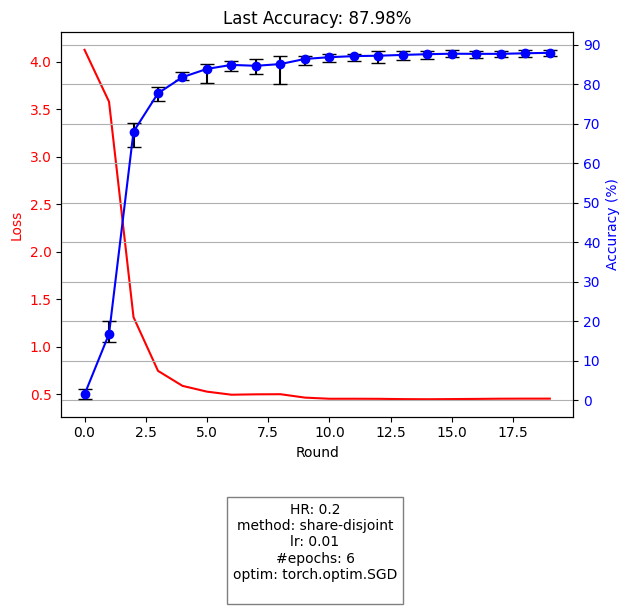
\includegraphics[width=0.8\textwidth]{../plots/femnist-horizontal/sgd/results-h0_2-hm_share-disjoint-lr0_01-e6-torch_optim_SGD.png}  % Adjust width as needed
                \caption{Caption describing the image}
                \label{fig:femnists2sgd}
            \end{figure}rnel_size=3,
            padding=1
        )
        self.conv2 = nn.Conv2d(
            in_channels=32,
            out_channels=64,
            kernel_size=3,
            padding=1,
        )
        # fully connected layer
        self.fc = nn.Linear(64 * 7 * 7, 512)
        # output layer
        self.classification = nn.Linear(512, num_classes)

    def forward(self, x):
        x = self.pool(F.relu(self.conv1(x)))
        x = self.pool(F.relu(self.conv2(x)))
        # flatten
        x = x.view(-1, 64 * 7 * 7)
        x = F.relu(self.fc(x))
        out = F.log_softmax(self.classification(x), dim=1)
        return out
\end{lstlisting}


\subsubsection{HAR HFL - MLP}
Il modello utilizzato per l'UCI HAR a partizionamento orizzontale 
è una semplice rete neurale composta di soli layer fully connected 
con un solo hidden layer. Ha un input per le 561 feature, un output 
di 6 neuroni per le 6 classi e un piccolo layer intermedio di 50 neuroni.
Nonostante le dimensioni ridotte del modello (28406 parametri totali)
si è riusciti comunque ad ottenere ottime prestazioni (> 90\%),
dimostrando la validità dell'approccio anche in contesti a risorse
ridotte, come telefoni o dispositivi IoT. Questa simulazione è stata 
anche eseguita interamente in CPU, senza accelerazione GPU, perché 
dato la maggiore quantità di RAM (32GB di RAM contro 6GB di VRAM
sulla GPU) sulla macchina usata per gli esperimenti, si è riusciti a 
terminare la simulazione più velocemente data la maggiore possibilità
di parallelizzazione del training svolto dai client. L'implementazione
di questo modello in PyTorch è la seguente:

\begin{lstlisting}
class HarModel(nn.Module):
    def __init__(self, num_classes: int):
        super(HarModel, self).__init__()
        self.fc1 = nn.Linear(561, 50)
        self.fc2 = nn.Linear(50, num_classes)

    def forward(self, x):
        x = F.relu(self.fc1(x))
        out = F.log_softmax(self.fc2(x), dim=1)
        return out
\end{lstlisting}


\subsubsection{HAR VFL - MLP distribuito}
In ultimo è stato anche provato un modello a partizionamento verticale 
delle feature dell'UCI HAR. In questo contesto, dati \(K\) client,
ogni modello di un client prende \(561/K\) feature e calcola un encoding 
di queste in un vettore dimensione \(d\). Le dimensioni del vettore 
provate sono state \(d=10\) e \(d=100\). Calcolati gli encodings, 
il server raccoglie \(K\) di questi encodings in unico vettore di lunghezza
\(Kd\). Questo vettore di encodings viene poi passato ad un ultima rete 
neurale fully connected con un layer nascosto di 50 neuroni e 
l'output è di nuovo un vettore di dimensione 6 per le 6 attività. Il 
modello dei client è stato implementato con il codice seguente:

\begin{lstlisting}
class ClientVerticalModel(nn.Module):
    def __init__(self, num_features: int):
        super(ClientVerticalModel, self).__init__()
        self.input = nn.Linear(num_features, 50)
        self.latent = nn.Linear(50, latent_vector_length)

    def forward(self, x):
        x = F.relu(self.input(x))
        latent = F.relu(self.latent(x))
        return latent
\end{lstlisting}

Mentre il codice per la rete del server che raccoglie gli encodings e 
calcola la classificazione dell'input è:

\begin{lstlisting}
class ServerVerticalModel(nn.Module):
    def __init__(self, num_clients, num_classes: int):
        super(ServerVerticalModel, self).__init__()
        self.input = nn.Linear(num_clients * latent_vector_length, 50)
        self.output = nn.Linear(50, num_classes)

    def forward(self, x):
        x = F.relu(self.input(x))
        out = F.log_softmax(self.output(x), dim=1)
        return out
\end{lstlisting}

Per comodità in fase di testing del modello è stato anche implementata 
una versione unica del modello, in grado di prendere le 561 feature e 
calcolare la classificazione direttamente, facendo uso dei modelli 
client e del modello server passati nel costruttore. Dato che può 
facilitare a comprendere meglio il funzionamento del VFL di seguito è
riportato anche il codice di questo modello:

\begin{lstlisting}
class FullVerticalModel(nn.Module):
    def __init__(
        self,
        client_models: list[ClientVerticalModel],
        server_model: ServerVerticalModel,
        num_clients: int,
    ):
        super(FullVerticalModel, self).__init__()
        self.client_models = client_models
        self.server_model = server_model
        self.num_clients = num_clients

    def forward(self, x):
        embeddings = []
        for cid, model in enumerate(self.client_models):
            extracted_features = extract_features(x, self.num_clients, cid)
            embeddings.append(model(extracted_features))

        embeddings_aggregated = torch.cat(embeddings, dim=1)
        return self.server_model(embeddings_aggregated)
\end{lstlisting}


Ognuno di questi modelli è stato allenato con Cross Entropy Loss
come loss function e con due diversi algoritmi di 
ottimizzazione.
Il primo provato è il classico SGC (Stochastic Gradient
Descent) con learning rate di 0.01 e momentum di 0.9. Esperimenti
preliminari hanno provato altri valori come un learning rate più basso
come 0.001 o più grande come 0.1 o la rimozione del momentum, ma le 
performance migliori sono state ottenute con i valori indicati 
precedentemente; la CNN per il FEMNIST non riusce nemmeno a convergere 
senza momentum e l'accuracy sul test dataset si ferma intorno al 6\%.
L'altro algoritmo usato è stato l'AdamW ~\cite{Loshchilov2017AdamW}, 
ovvero l'algoritmo Adam (Adaptive Movement Estimation) con weight 
decay. In esperimenti preliminari è anche stato provato l'Adam classico 
ma si è notato che sia il loss che la test accuracy erano molto 
instabili durante il training, suggerendo suggerendo che i parametri 
del modello fossero altrettanto instabili. Per tale motivo si è 
scelto di utilizzare la variante AdamW che implementa il weight decay 
come meccanismo di regolarizzazione per mantere i pesi del modello più
stabili. Si noti che si è evitato esplicitamente di utilizzare una 
L\sub{2} regularization come loss function per risolvere l'instabilità 
di Adam, dato che la L\sub{2} regularization e il weight decay sono 
equivalenti solo sotto SGD ~\cite{Loshchilov2017AdamW}.

\subsection{Ibridazione}
Per gli esperimenti a partizionamento orizzontale si sono fatti 
esperimenti per diversi gradi di ibridazione da simulazione completamente
federate a simulazioni completamente centralizzate. La configurazione 
dello script di training ammette due paramerti per controllare il grado 
di ibridazione da usare: \texttt{hybrid\_ratio} e 
\texttt{hybrid\_method}, che controllano
rispettivamente la percentuale dei dataset dei client da condividere in 
un unico dataset globale e il meccanismo di condivisione dei dataset.
Le tecniche di condivisione implementate sono state chiamate \texttt{unify}
e \texttt{share-disjoint}. Nel caso della \texttt{share-disjoint} ogni
client 
prende la percentuale indicata di sample dal suo dataset e li sposta
nel dataset condiviso, mentre nella \texttt{unify} la percentuale 
indicata di 
client condividono il loro dataset intero. Ad esempio, supponendo di 
avere 10 client con 10 dataset che contengono tutti 100 sample con un 
\texttt{hibrid\_ratio} di 0.2, con la \texttt{share-disjoint} ognuno 
dei 10 client prende
20 sample dal suo dataset e li mette nel dataset condiviso, ottenento 
un dataset condiviso di 200 sample e 10 client con 80 sample ciascuno,
mentre nella \text{unify} vengono selezionati randomicamente 2 client che 
condividono tutti i loro 100 sample, ottenendo un dataset condiviso di 
200 sampe e 8 client con 100 sample ciascuno.

Il codice che segue è il codice utilizzato per condividere parte dei 
dataset dei client, una volta che i dataset sono stati istanziati già
partizionanti per client:

\begin{lstlisting}
def _centralize_trainsets(
    train_sets: list[Dataset], num_clients: int, hybrid_ratio, hybrid_method
):
    if hybrid_method == "unify":
        num_centralized = int(hybrid_ratio * num_clients)
        shared_sets = []
        for _ in range(num_centralized):
            random_index = random.randint(0, len(train_sets) - 1)
            shared_sets.append(train_sets.pop(random_index))

        if num_centralized > 0:
            train_sets = [ConcatDataset(shared_sets)] + train_sets

    elif hybrid_method == "share-disjoint":
        # this method removes num_shared samples from clients and puts them in the collective
        shared_sets = []
        client_sets = []
        for train_set in train_sets:
            set_size = len(train_set)
            num_shared = int(hybrid_ratio * set_size)
            if num_shared > 0:
                shared_set, unshared_set = random_split(
                    train_set, [num_shared, set_size - num_shared]
                )
                shared_sets.append(shared_set)
                client_sets.append(unshared_set)
            else:
                # dont lose clients sets!
                client_sets.append(train_set)
        if len(shared_sets) > 0:
            train_sets = client_sets + [ConcatDataset(shared_sets)]

    return train_sets
\end{lstlisting}

\chapter{Risultati}
In questo capitolo vengono presentati i risultati degli esperimenti 
condotti. Il capitolo è diviso in tre sezioni.
Le prime due sezioni, una per dataset studiato, hanno la stessa 
struttura: il primo paragrafo sintetizza il 
setup dell'esperimento presentato e discute anche qualche esperimento
preliminare condotto che ha portato alla decisione di alcuni parametri.
In ultimo, la sezione finale discute possibili miglioramenti al setup
utilizzato in questo studio.


\section{FEMNIST}
In questa sezione vengono descritti gli esperimenti fatti con il dataset
FEMNIST e vengono descritti i risultati.

\subsection{Set up}
Come già anticipato, gli esperimenti sul dataset FEMNIST sono stati fatti 
utilizzando una CNN con 2 layer convoluzionali con 32 e 64 canali di 
output, seguiti da un layer lineare con 512 neuroni. Si sono provate le 
strategie di ibridazione \texttt{unify} e \texttt{share-disjoint},
condividendo i dataset selezionando alcuni client i cui dataset 
vengono interamente condivisi oppure prendendo una parte di sample da 
ogni dataset locale, mentre come gradi di ibridazione si è andati da 0\%,
completamente federato, al 100\%, completamente centralizzato,
in step di 10\%. Gli algoritmi di ottimizzazione provati sono SGD 
con learning rate \(\eta = 0.01\) e momentum \(\beta = 0.9\) e l'AdamW
con learning rate \(\eta = 0.01\). Il training ha usato 6 epoche locali
ed è durato per 20 round. Sono stati usati i sample di soltanto 100 
scrittori del totale presenti nel FEMNIST. I risultati presentati 
successivamente sono una media su 20 simulazioni.

Oltre ai risultati di questo esperimento, presentati nel paragrafo
successivo, sono stati fatte anche simulazioni preliminari con 
iperparametri diversi. Primo fra tutti è il numero di client, che negli 
esperimenti finali è stato mantenuto basso per velocizzare il processo 
di training, mentre sono state eseguite simulazioni fino a 1000 client 
utilizzati. Il numero poi stato mantenuto basso perché in tutti gli 
esperimenti fatti i risultati ottenuti erano sempre gli stessi, 
indipendentemente dal numero di client che partecipavano.
Un'altra risultato interessante è stato l'esperimento utilizzando SGD
senza momentum, in cui si è visto che la CNN non è riuscita a imparare,
mantenendo un accuracy sul dataset di test intorno al 6\%.

\subsection{Risultati}
Il dataset FEMNIST è quello dei due che si è dimostrato più difficile 
da imparare e su cui è più notevole il miglioramento di performance 
dato dalla condivisione dei dati (circa il 10\% dal setting totalmente
federato a quello totalmente centralizzato). La figura \ref{fig:femnistrandom}
mostra i risultati del training ai due estremi di ibridazione:
\ref{fig:femnistrandoma} mostra i risultati dell'apprendimento federato,
mentre \ref{fig:femnistrandomb} quelli dell'apprendimento centralizzato.
\begin{figure}[hb]  % h: here, t: top, b: bottom, p: page
    \centering
    \begin{subfigure}[b]{0.49\textwidth}
        \centering
        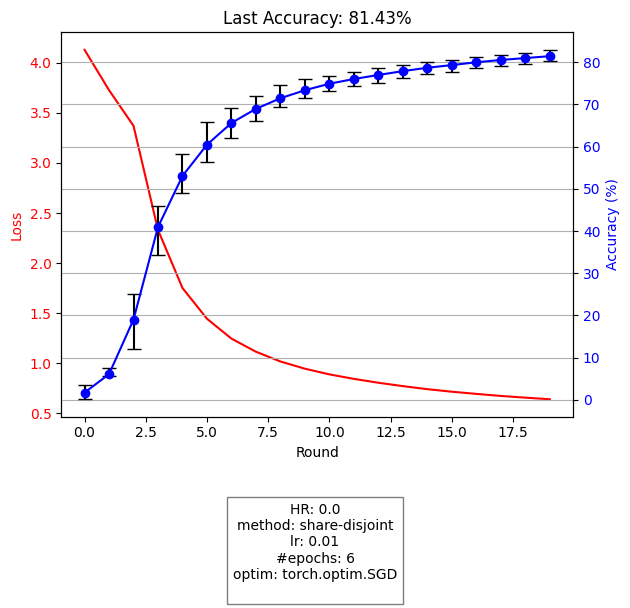
\includegraphics[width=\textwidth]{../plots/femnist-horizontal/sgd/results-h0_0-hm_share-disjoint-lr0_01-e6-torch_optim_SGD.png}
        \caption{Federato}
        \label{fig:femnistrandoma}
    \end{subfigure}
    \hfill
    \begin{subfigure}[b]{0.49\textwidth}
        \centering
        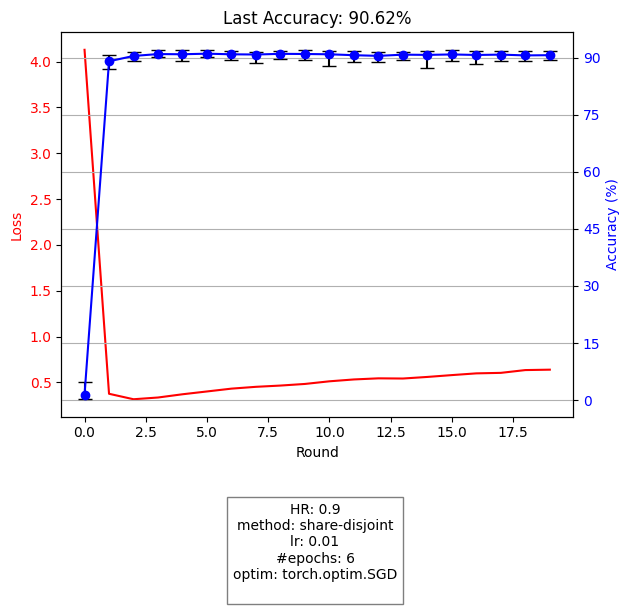
\includegraphics[width=\textwidth]{../plots/femnist-horizontal/sgd/results-h0_9-hm_share-disjoint-lr0_01-e6-torch_optim_SGD.png}
        \caption{Centralizzato}
        \label{fig:femnistrandomb}
    \end{subfigure}
    
    \caption{
        Risultati del del training per ogni round. A sinistra (a) si può 
        vedere l'apprendimento federato, a destra (b) quello centralizzato.
        Algoritmo di ottimizzazione (SGD) e metodo di condivisione 
        (\texttt{share-disjoint}) sono tenuti fissati.
    }
    \label{fig:femnistrandom}
\end{figure}


Come si può vedere nel caso federato 
le performance raggiungono una precisione del 81.43\% sul testset 
e si può anche notare che il modello non è ancora arrivato a convergenza.
Continuando il training per ulteriori round possiamo quindi aspettarci 
di poter migliorare le prestazioni ancora.
Il modello centralizzato arriva ad un'accuracy maggiore di un 9\% e 
soprattutto bastano 2 round per ottenere risultati sopra al 90\%.

Un primo caso di chiara convergenza intorno all'88\% lo si vede quando 
si inizia a condividere il 20\% dei dataset come mostrato in figura 
\ref{fig:femnists2sgd}, dove si può vedere che l'accuracy del modello 
smette di migliorare intorno al decimo round.
\begin{figure}[hb]  % h: here, t: top, b: bottom, p: page
    \centering
    \begin{subfigure}[b]{0.49\textwidth}
        \centering
        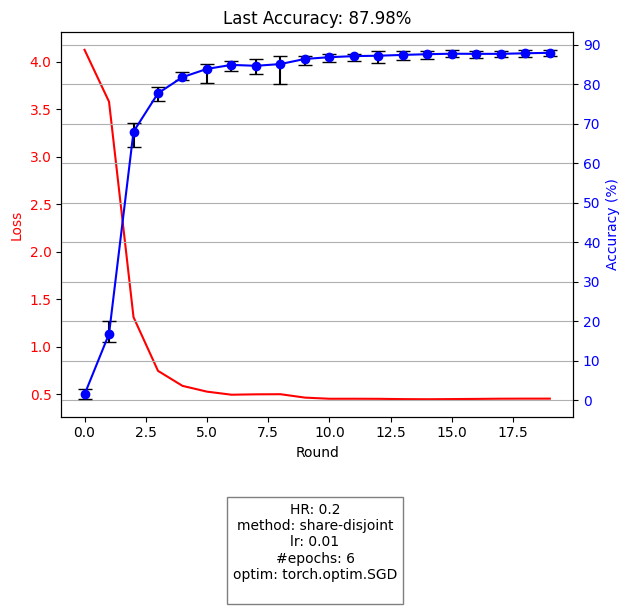
\includegraphics[width=\textwidth]{../plots/femnist-horizontal/sgd/results-h0_2-hm_share-disjoint-lr0_01-e6-torch_optim_SGD.png}
        \caption{\texttt{share-disjoint} con ibridazione 20\%}
        \label{fig:femnists2sgd}
    \end{subfigure}
    \hfill\begin{subfigure}[b]{0.49\textwidth}
        \centering
        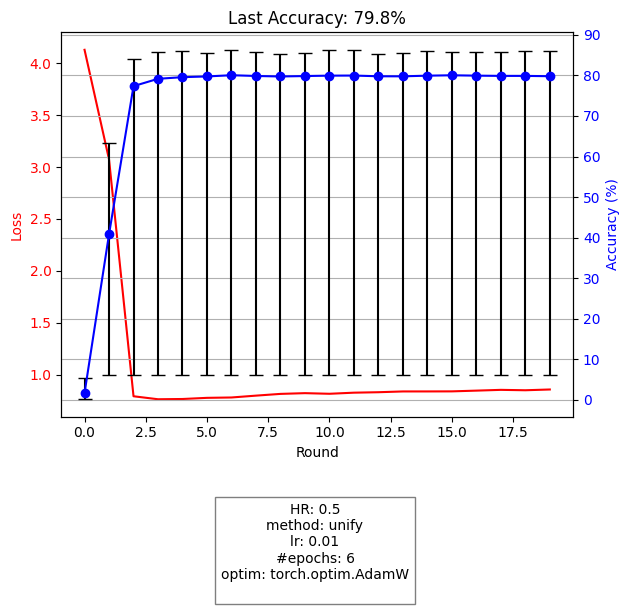
\includegraphics[width=\textwidth]{../plots/femnist-horizontal/adamw/results-h0_5-hm_unify-lr0_01-e6-torch_optim_AdamW.png}
        \caption{\texttt{unify} con ibridazione 50\%}
        \label{fig:feministu5adam}
    \end{subfigure}
    
    \caption{
        Risultati del training diversi. Il grafico a sinitra (a) 
        mostra i risultati di una condivisione \texttt{share-disjoint}
        al 20\%, mentre quello a destra (b) usa il metodo 
        \texttt{unify} al 50\%.
    }
    \label{fig:femnistadam}
\end{figure}

Dei due ottimizzatori provati, SGD è quello che performa meglio: è più 
veloce nell'apprendimento, ottiene performance migliori alla fine del 
training ed è molto più stabile. In particolare tutte le run che hanno 
utilizzato AdamW e il metodo di condivisione \texttt{unify} mostrano 
sempre intervalli di incertezza enormi, come quello riportato in 
figura \ref{fig:feministu5adam}. La situazione è analoga anche usando 
la condivisione \texttt{share-disjoint} fino a che il grado di 
condivisione non raggiunge un minimo del 40\%, come mostrato nelle 
figure \ref{fig:feminists3adam} e \ref{fig:feminists4adam}, e anche 
dopo oltre il 40\% non è garantita una maggiore stabilità, come ha 
rivelato l'esperimento con 80\% di condivisione (figura \ref{fig:feminists8adam}).
\begin{figure}[htbp]  % h: here, t: top, b: bottom, p: page
    \centering
    \begin{subfigure}[b]{0.49\textwidth}
        \centering
        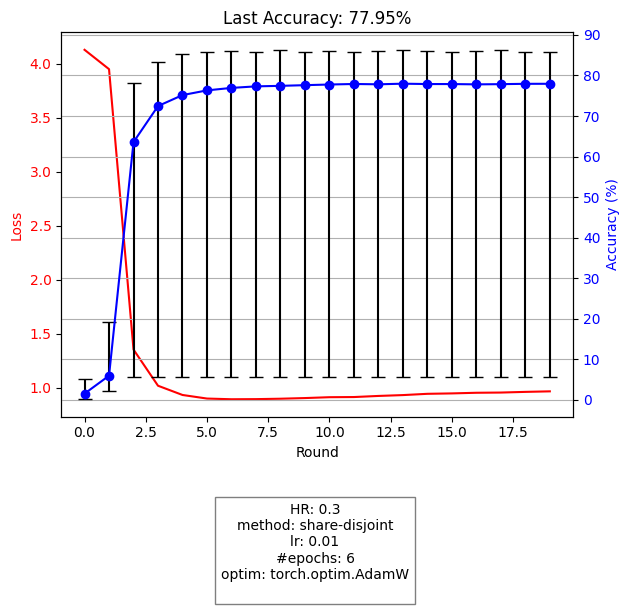
\includegraphics[width=\textwidth]{../plots/femnist-horizontal/adamw/results-h0_3-hm_share-disjoint-lr0_01-e6-torch_optim_AdamW.png}
        \caption{Figura 5.3(a)}
        \label{fig:feminists3adam}
    \end{subfigure}
    \hfill
    \begin{subfigure}[b]{0.49\textwidth}
        \centering
        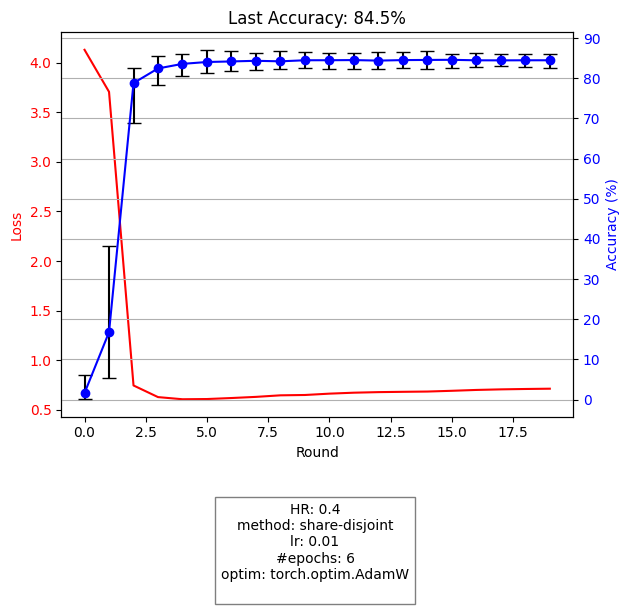
\includegraphics[width=\textwidth]{../plots/femnist-horizontal/adamw/results-h0_4-hm_share-disjoint-lr0_01-e6-torch_optim_AdamW.png}
        \caption{Figura 5.3(b)}
        \label{fig:feminists4adam}
    \end{subfigure}
    \centering
    \begin{subfigure}[b]{0.49\textwidth}
        \centering
        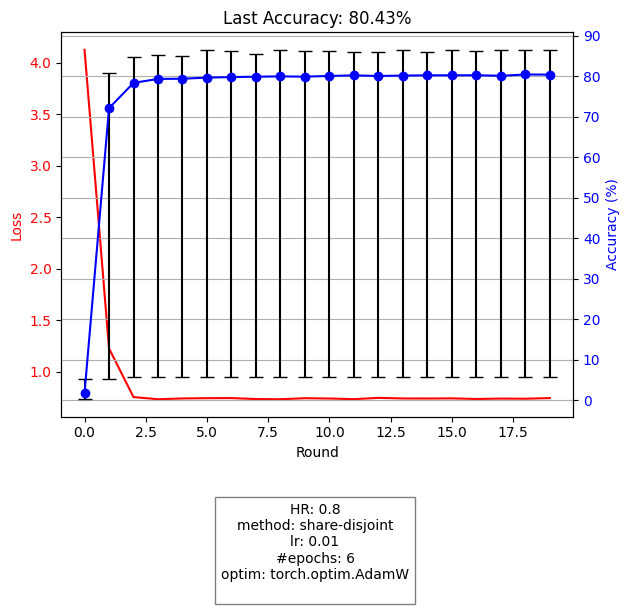
\includegraphics[width=\textwidth]{../plots/femnist-horizontal/adamw/results-h0_8-hm_share-disjoint-lr0_01-e6-torch_optim_AdamW.png}
        \caption{Figura 5.3(c)}
        \label{fig:feminists8adam}
    \end{subfigure}
    
    \caption{
        Diversi risultati di training con AdamW e metodo \texttt{share-disjoint}.
        Il primo (a) usa una condivisione del 30\%, il secondo (b) al 40\%
        il minimo per cui AdamW ha un andamento stabile, l'ultimo (c) 
        mostra un altro training instabile con condivisione all'80\%.
    }
    \label{fig:femnistsxtm}
\end{figure}

Guardando questi grafici si può notare come il comportamento medio non sia 
necessariamente rappresentativo di tutti i modelli allenati con AdamW, dato 
l'ampio margine d'incertezza e si potrebbe pensare che, al di là dei problemi 
di instabilità sia comunque possibile ottenere un modello performante
utilizzando quest'algoritmo. Va però notato che comunque anche i modelli 
meglio performanti allenati con AdamW, non hanno raggiunto performance 
superiori né uguali a quelle ottenute con SGD, con massimo di 90.69\%
(mediamente) per SGD, contro un 86\% circa di massimo totale.

Un'ultima osservazione che può essere fatta è come il metodo di condivisione
\texttt{share-disjoint} sia generalmente più stabile rispetto al 
\texttt{unify}. La spiegazione è semplice: \texttt{unify} scegliendo 
certi client da scegliere come dataset condivisi crea un dataset 
globale che conterrà gli stessi bias presenti nei dataset dei client 
selezionati; \texttt{share-disjoint} invece, selezionando alcuni sample 
da tutti i dataset locali, garantisce di coprire, almeno in parte, 
tutte le peculiarità nei dati di tutti i client. In questo dataset 
questo effetto non è particolarmente marcato se non con l'AdamW o nei 
primissimi round di training con basso gradi di condivisione in SGD.

In conclusione, si è osservato come la condivisione di un numero ristretto 
di dati potra ad un miglioramento delle prestazioni apprezzabile: passare 
dal condividere lo 0\% al 10\% di dati si ottiene un miglioramento di 
circa 5\% di accuracy e passare dal 10\% al 20\% comporta un miglioramento
di un ulteriore 2/3\%, portando le prestazioni finali all'88\%, 
risultato comparabile con il 90\% ottenuto sul training centralizzato.
Oltre il 30\% di condivisione i miglioramenti che si ottengono sono 
sempre più marginali e non superano l'1\%, suggerendo il 20\% come un 
buon compromesso tra performance e condivisione dei dati.
La strategia \texttt{share-disjoint} permette inoltre un training più
stabile, fattore che si è rivelato molto importante negli esperimenti
con ottimizzatore AdamW, altra fonte di instabilità.

Nell'appendice A si può trovare l'elenco dei grafici di tutti gli 
esperimenti condotti sul FEMNIST.
    

\clearpage
\section{HAR - HFL}
In questa sezione vengono descritti gli esperimenti fatti con il dataset
UCI HAR con il normale partizionamento orizzontale e vengono descritti 
i risultati.

\subsection{Set up}
Per l'UCI HAR invece è stata utilizzata una semplice MLP con un solo 
hidden layer di 50 neuroni. Di nuovo, si sono provate le 
strategie di ibridazione \texttt{unify} e \texttt{share-disjoint} con 
gradi di ibridazione da 0\% a 100\% in passi di 10\%. Anche qui sono 
stati testati sia l'ottimizzatore SGD che AdamW con learning rate 
\(\eta = 0.01\) e momentum \(\beta = 0.9\) nel caso di SGD. Il 
training ha usato 5 epoche locali, è durato 20 round e i risultati 
sono una media su 20 simulazioni consecutive. In questo caso è stato 
utilizzato l'intero dataset con 30 diversi client.

In esperimenti preliminari anche con questo dataset si è provato ad 
utilizzare SGD senza momentum e in questo caso il modello è stato in 
grado di convergere lo stesso, seppur rallentando prevedibilmente 
l'apprendimento. Sono stati provati anche valori diversi di learning 
rate come \(\eta = 0.1\) o \(\eta = 0.001\) ma non si sono viste 
differenze interessanti nell'apprendimento, se non una leggera 
instabilità maggiore o una velocità di apprendimento minore.
Inoltre i primi modelli provati erano di dimensioni più grandi. 
Tuttavia, viste fin dall'inizio le ottime prestazioni ottenute su 
questo dataset si è ridotto il modello ad un unico layer nascosto di 
soli 50 neuroni.


\subsection{Risultati}
L'UCI HAR è il dataset che ha mostrato le performance migliori.
Innanzitutto nonostante la dimensione piuttosto contenuta del modello
utilizzato si è riusciuti ad avere ottime prestazioni lo stesso, non 
scendendo mai al di sotto del 90\% di accuracy e avvicinandosi al 
95\% per gli esperimenti con maggior grado di ibridazione. Le 
figure \ref{fig:hars0sgd} e \ref{fig:hars9sgd} mostrano i risultati 
ai due estremi di ibridazione.
Come si può vedere anche in questo caso il modello centralizzato 
richiede solo 2 round per superare il 50\% di accuracy e termina 
l'apprendimento intorno al quinto round. Il modello federato invece
richiede ben più round di training, superando il 90\% intorno al 
quindicesimo round e termina con un 91.15\%.

\begin{figure}[htp]  % h: here, t: top, b: bottom, p: page
    \centering
    \begin{subfigure}[b]{0.49\textwidth}
        \centering
        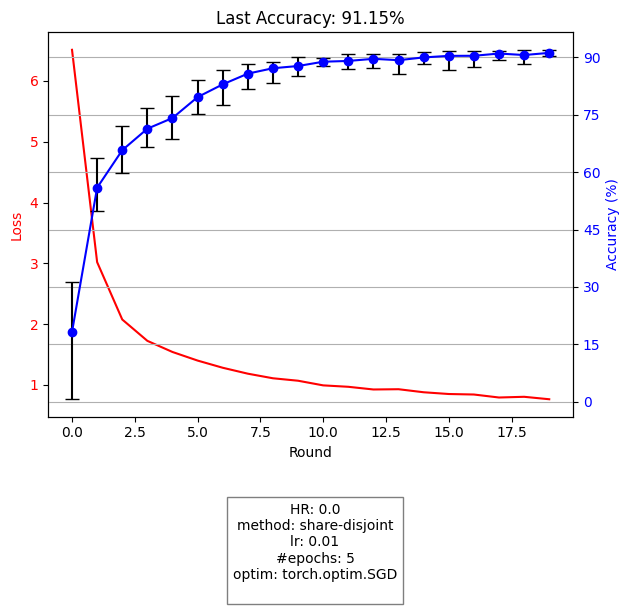
\includegraphics[width=\textwidth]{../plots/har-horizontal/sgd/results-h0_0-hm_share-disjoint-lr0_01-e5-torch_optim_SGD.png}
        \caption{0\% Condivisione}
        \label{fig:hars0sgd}
    \end{subfigure}
    \hfill
    \begin{subfigure}[b]{0.49\textwidth}
        \centering
        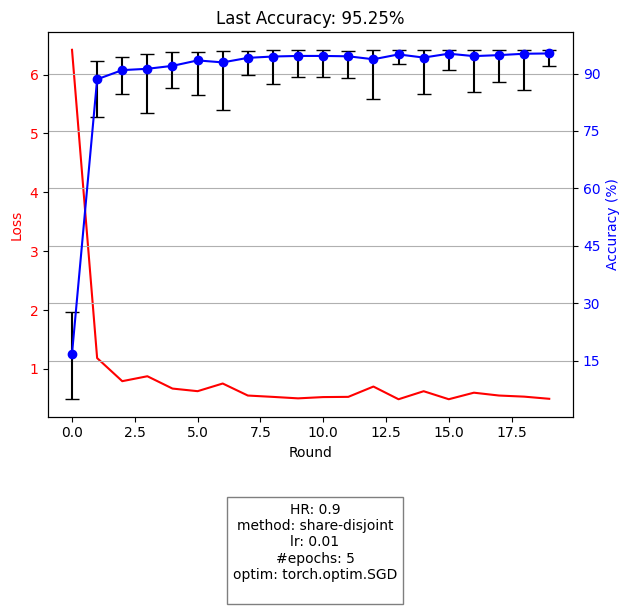
\includegraphics[width=\textwidth]{../plots/har-horizontal/sgd/results-h0_9-hm_share-disjoint-lr0_01-e5-torch_optim_SGD.png}
        \caption{100\% Condivisione}
        \label{fig:hars9sgd}
    \end{subfigure}
    
    \caption{
        Risultati del training per ogni round. A sinistra (a) si può 
        vedere l'apprendimento federato, a destra (b) quello centralizzato.
        Algoritmo di ottimizzazione (SGD) e metodo di condivisione 
        (\texttt{share-disjoint}) sono tenuti fissati.
    }
\end{figure}


Una differenza interessante rispetto al FEMNIST è che in questo 
caso AdamW si comporta sensibilmente meglio. Tanto per cominciare
le performance dei modelli allenati con SGD sono perfettamente 
comparabili a quelle dei modelli allenati con AdamW, anziché 
performare peggio. Inoltre AdamW mostra una maggiore resistenza 
all'instabilità dell'apprendimento provocata dalla condivisione 
dei dataset con il metodo \texttt{unify}. In figura 
\ref{fig:haru6sgd} si può vedere il risultato del training con SGD,
metodo \texttt{unify} al 60\% di condivisione, mentre in figura 
\ref{fig:haru6adam} si vede il risultato del training sotto le 
stesse condizioni usando l'algoritmo AdamW. Come si può vedere 
dagli intervalli di incertezza AdamW risulta più stabile in 
queste condizioni.
\begin{figure}[htp]  % h: here, t: top, b: bottom, p: page
    \centering
    \begin{subfigure}[b]{0.49\textwidth}
        \centering
        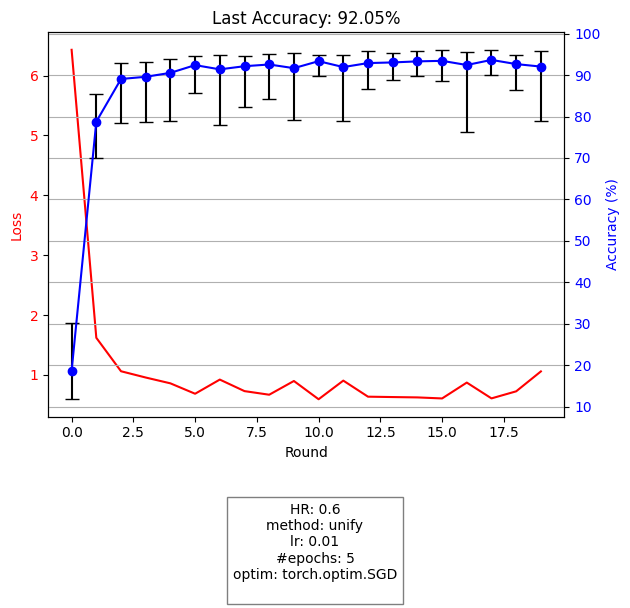
\includegraphics[width=\textwidth]{../plots/har-horizontal/sgd/results-h0_6-hm_unify-lr0_01-e5-torch_optim_SGD.png}
        \caption{Training con SGD}
        \label{fig:haru6sgd}
    \end{subfigure}
    \hfill
    \begin{subfigure}[b]{0.49\textwidth}
        \centering
        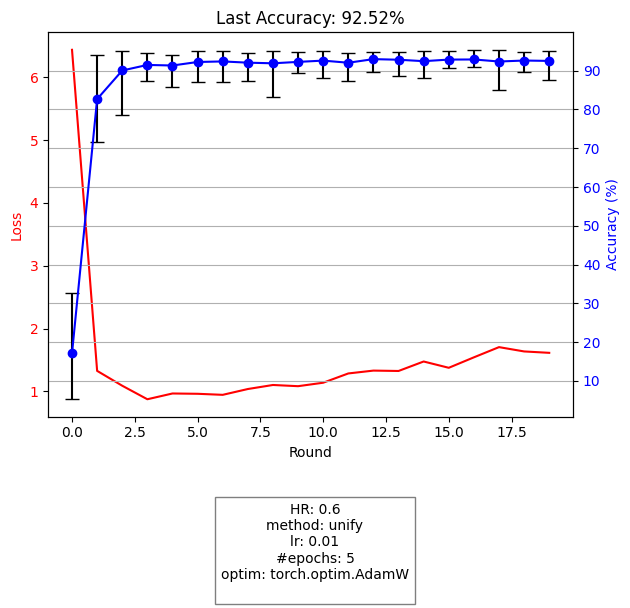
\includegraphics[width=\textwidth]{../plots/har-horizontal/adam/results-h0_6-hm_unify-lr0_01-e5-torch_optim_AdamW.png}
        \caption{Training con AdamW}
        \label{fig:haru6adam}
    \end{subfigure}
\end{figure}

Concludendo quest'analisi, anche in questo si è potuto riscontrare
un effettivo miglioramento di performance all'aumentare dell'ibridazione,
seppur con margini più stretti, in quanto l'accuracy del modello 
federato è già piuttosto alta. Passando da condivsione nulla ad allenamento
centralizzato si ottiene un miglioramento complessivo di circa 5 punti 
percentuali. Anche in questo caso con una condivisione del 20\% si può 
ottenere la maggior parte di questo miglioramento e con una condivisione 
del 40\% si ottengono risultati davvero simili a quelli del modello 
centralizzato (94.5\% contro un 95.25\% per il centralizzato).

Tutti i grafici degli esperimenti sull'UCI HAR sono nell'appendice B

\clearpage
\section{HAR - VFL}
L'ultimo esperimento fatto è quello del UCI HAR con partizionamento 
verticale delle feature.

In questo caso la rete neurale che compie la classificazione è 
distribuita tra client e server. Dato un numero di client \(K\) 
configurabile ogni ogni client ha un MLP che accetta \(561 / K\)
feature (dove l'utlimo client prende le feature rimanenti in caso di 
resto diverso da 0) e ne calcola un encoding. Sono state provate due 
dimensioni diverse di encoding: su un vettore lungo 10 e lungo 100.
Data la lunghezza \(l\) del vettore di encoding, il server ha un'altra 
MLP che accetta un vettore lungo \(Kl\) e ne calcola la classificazione.
Sia il modello dei client che quello del server hanno un hidden layer 
di 50 neuroni.

I risultati di questo esperimento sono stati però deludenti: a discapito
di quale ottimizzatore venisse utilizzato tra SGD e AdamW, del numero di client da 
3 a 50 e della dimensione dell'encoding non si è mai riusciti ad ottenere 
un'accuracy superiore al 18\%, rimanendo quindi appena sopra
1 / 6 = 16.7\% cioè la probabilità di prenderci tirando a caso ogni 
volta su 6 classi. Si può quindi concludere che questo partizionamento
delle feature su questo dataset non è un approccio funzionante.


\section{Possibili sviluppi futuri}
Come già accennato, questo studio non ha l'obbiettivo di ottenere le 
migliori prestazioni possibili e come tale offre un ampio margine di 
miglioramento, specie nel caso in cui queste stesse tecniche vengano 
applicate a problemi più complessi.  


\subsubsection{Funzioni di attivazione}
Un primo possibile miglioramento 
è quello di cambiare alcuni parametri 
della rete neurale.
La funzione di attivazione ReLU, ad esempio, è 
estremamente popolare ed efficace nel mitigare il problema del 
vanishing gradient, ma anch'essa ha le sue limitazioni come il 
problema del \textit{dying ReLU}. Alternative che possono essere 
esplorate sono la Leaky ReLU (LReLU) ~\cite{Maas2013RectifierNI},
definita come
\[
LReLU(z) = 
\begin{cases} 
      z, & \text{se } z > 0 \\
      \alpha z, & \text{altrimenti}
\end{cases}
\]
che ammette valori diversi da 0 per argomenti negativi e introduce un 
altro iperparametro \(\alpha\), tipicamente piccolo,
o la Parametric ReLU (PReLU) che rende l'iperparametro \(\alpha\)
un parametro \(a_i\) da imparare per ogni neurone:
\[
PReLU(z_i) = 
\begin{cases} 
      z_i, & \text{se } z_i > 0 \\
      a_i z_i, & \text{altrimenti}
\end{cases}
\]
Altre varianti della ReLU interessanti, in quanto funzioni liscie e 
differenziabili anche su 0, sono la Gaussian Error Linear Units (GELU)
~\cite{hendrycks2016gelu}
\[
GELU(z) = z P(Z \le z) = z \Phi(z)
\]
o la Exponential Linear Unit (ELU) ~\cite{clevert2016elu}, 
che assume anche valori negativi fino a -1
\[
ELU(z) = 
\begin{cases} 
      z, & \text{se } z > 0 \\
      \alpha (e^z - 1), & \text{altrimenti}
\end{cases}
\]
per un qualche iperparametro \alpha < 0.


\subsubsection{Regolarizzazione}
In questi esperimenti non si è fatto particolare uso di tecniche di 
normalizzazione o regolarizzazione, se non per una normalizzazione 
applicata alla immagini del FEMNIST ottenuta dalle trasformazioni 
built-in fornite da PyTorch. Si potrebbe allora provare alcune di 
queste tecniche come l'utilizzo della normalizzazione \(L_2\) in caso si 
usi SGD (\(L_2\) e weight decay sono equivalenti solo sotto SGD 
~\cite{Loshchilov2017AdamW}) oppure una delle varie tecniche di 
normalizzazione che velocizzano il training riducendo l'effetto del 
\textit{covariate shift}, come la batch normalization ~\cite{ioffe2015batch},
la layer normalization ~\cite{ba2016layer} o la group normalization 
~\cite{wu2018group}


\subsubsection{Scaling Up}
Un altro metodo efficace per migliorare le performace di una rete neurale 
è quello di scalare le dimensioni del modello, dei dataset o del training.
Operare con un'ampia mole di utenti e quindi con molte fonti di dati,
far produrre più dati per il training ove possibile o rendere i modelli 
più complessi possono essere opzioni percorribili. Bisogna tenere in 
considerazione il fatto che modelli più grandi possono incappare nel 
problema dell'overfitting, richiedere più risorse computazionali, 
rischiando di tagliare fuori alcuni dispositivi meno performati, e 
aumenta l'utilizzo della banda di rete per la comunicazione di un 
maggior numero di parametri.


\subsubsection{Inductive Bias migliori}
Un'altra recente area di studio nel campo del deep learning è quella 
della ricerca di architetture che per come sono costruite implementano
strutturalmente un'invarianza desiderata a qualche trasformazione 
dell'input. Un esempio concreto è l'invarianza traslazionale che 
implementano i layer convoluzionali attraverso la condivisione dei pesi.
Il geometric deep learning ~\cite{bronstein2021geometric} è lo studio di simmetrie 
(i.e. invarianti o equivarianti) geometriche che possono essere sfruttate nella 
progettazione di architetture neurali.
Il FEMNIST è un dataset particolare in cui tutti i caratteri sono stati
centrati e riscalati per ricoprire tutti la stessa area, cosa che in 
generale nella scrittura naturale è lontana dalla realtà. Può essere 
interessante esplorare architetture convoluzionali che siano invarianti 
anche a rotazioni o rescaling ~\cite{sosnovik2023symmetry, cohen2016group,
marcos2016rotation, cohen2016steer}.

Rimane però il fatto che le simmetrie desiderate dipendono fortemente 
dal problema trattato e per tale ragione vanno analizzate per lo 
specifico problema preso in considerazione.


\subsubsection{Data Augmentation}
Un altro metodo per \textit{insegnare} ad un modello ad essere invariante
a certe trasformazioni come la rotazione è quello del data augmentation.
In questo caso quello che si può fare è produrre nuovi dati da fornire
al modello nel training, facendo delle trasformazioni sui dati 
originali (come appunto rotare le immagini, aggiungere noise artificiale,
invertire le immagini...) o anche producendo dati sintetici del tutto
nuovi. Nell'era dei modelli generativi infatti, un'ulteriore possibilità
è quella di far generare dei dati del tutto sintetici ad un modello 
generativo che abbiano la stessa distribuzione dei dati naturali.

Bisogna però tenere presente che questo approccio non è efficace nel 
risolvere il problema della \textit{curse of dimensionality}
~\cite{bellman1957dynamic, Hughes1968OnTM, bronstein2021geometric}, 
per cui il numero di data points nel training set scala esponenzialmente 
in funzione della dimensionalità dell'input della funzione che 
cerchiamo di apprendere.

\chapter{Miglioramenti}
Come già accennato, questo studio non ha l'obbiettivo di ottenere le 
migliori prestazioni possibili e come tale offre un ampio margine di 
miglioramento, specie nel caso in cui queste stesse tecniche vengano 
applicate a problemi più complessi.Un primo possibile miglioramento 
è quello di cambiare alcuni parametri 
della rete neurale. 


\subsubsection{Funzioni di attivazione}
La funzione di attivazione ReLU è 
estremamente popolare ed efficace nel mitigare il progblema del 
vanishing gradient, ma anch'essa ha le sue limitazioni come il 
problema del \textit{dying ReLU}. Alternative che possono essere 
esplorate sono la Leaky ReLU (LReLU) ~\cite{Maas2013RectifierNI},
definita come
\[
LReLU(z) = 
\begin{cases} 
      z, & \text{se } z > 0 \\
      \alpha z, & \text{altrimenti}
\end{cases}
\]
che ammette valori diversi da 0 per argomenti negativi e introduce un 
altro iperparametro \(\alpha\),
o la Parametric ReLU (PReLU) che rende l'iperparametro \(\alpha\)
un parametro \(a_i\) da imparare per ogni neurone:
\[
PReLU(z_i) = 
\begin{cases} 
      z_i, & \text{se } z_i > 0 \\
      a_i z_i, & \text{altrimenti}
\end{cases}
\]
Altre varianti della ReLU interessanti, in quanto funzioni liscie e 
differenziabili anche su 0, sono la Gaussian Error Linear Units (GELU)
~\cite{hendrycks2016gelu}
\[
GELU(z) = z P(Z \le z) = z \Phi(z)
\]
o la Exponential Linear Unit (ELU) ~\cite{clevert2016elu}, 
che assume anche valori negativi fino a -1
\[
ELU(z) = 
\begin{cases} 
      z, & \text{se } z > 0 \\
      \alpha (e^z - 1), & \text{altrimenti}
\end{cases}
\]
per un qualche iperparametro \alpha < 0.


\subsubsection{Regolarizzazione}
In questi esperimenti non si è fatto particolare uso di tecniche di 
normalizzazione o regolarizzazione, se non per una normalizzazione 
applicata alla immagini del FEMNIST ottenuta dalle trasformazioni 
built-in fornite da PyTorch. Si potrebbe allora provare alcune di 
queste tecniche come l'utilizzo della normalizzazione \(L_2\) in caso si 
usi SGD (\(L_2\) e weight decay sono equivalenti solo sotto SGD 
~\cite{Loshchilov2017AdamW}) oppure una delle varie tecniche di 
normalizzazione che velocizzano il training riducendo l'effetto del 
\textit{covariate shift}, come la batch normalization ~\cite{ioffe2015batch},
la layer normalization ~\cite{ba2016layer} o la group normalization 
~\cite{wu2018group}


\subsubsection{Scaling Up}
Un altro metodo efficace per migliorare le performace di una rete neurale 
è quello di scalare le dimensioni del modello, dei dataset o del training.
Operare con un'ampia mole di utenti e quindi con molte fonti di dati,
far produrre più dati per il training ove possibile o rendere i modelli 
più complessi possono essere opzioni percorribili. Bisogna tenere in 
considerazione il fatto che modelli più grandi possono incappare nel 
problema dell'overfitting, richiedere più risorse computazionali, 
rischiando di tagliare fuori alcuni dispositivi meno performati, e 
aumenta l'utilizzo della banda di rete per la comunicazione di un 
maggior numero di parametri.


\subsubsection{Inductive Bias migliori}
Un'altra recente area di studio nel campo del deep learning è quella 
della ricerca di architetture che per come sono costruite implementano
strutturalmente un'invarianza desiderata a qualche trasformazione 
dell'input. Un esempio concreto è l'invarianza traslazionale che 
implementano i layer convoluzionali attraverso la condivisione dei pesi.
Il geometric deep learning ~\cite{bronstein2021geometric} è lo studio di simmetrie 
(i.e. invarianti o equivarianti) geometriche che possono essere sfruttate nella 
progettazione di architetture neurali.
Il FEMNIST è un dataset particolare in cui tutti i caratteri sono stati
centrati e riscalati per ricoprire tutti la stessa area, cosa che in 
generale nella scrittura naturale è lontana dalla realtà. Può essere 
interessante esplorare architetture convoluzionali che siano invarianti 
anche a rotazioni o rescaling ~\cite{sosnovik2023symmetry, cohen2016group,
marcos2016rotation, cohen2016steer}.

Rimane però il fatto che le simmetrie desiderate dipendono fortemente 
dal problema trattato e per tale ragione vanno analizzate per lo 
specifico problema preso in considerazione.

\chapter{Conclusione}
In questo studio si è potuta verificare l'efficacia del 
federated learning ibrido. La condivisione di una piccola parte dei 
dataset locali può essere una strategia efficacie per affrontare le 
difficoltà poste dal federated learning.

I risultati dimostrano che condividere una parte dei dataset ha un 
effetto positivo apprezzabile sulle performance del modello. Sono stati 
considerati due dataset di due problemi fondamentalmente diversi -UCI HAR 
e FEMNIST- a confermare il fatto che i risultati non siano una particolarità
dello specifico problema o modello utilizzato. Il miglioramento di 
performance è stato particolarmente notevole nel FEMNIST che si è rivelato 
il dataset più complicato dei due. 

Tuttavia rimane importante bilanciare in modo appropriato la condivisione 
di dati, con la protezione della privacy ove necessario e informare 
l'utente della condivisione in atto, comportamento virtuoso anche in 
assenza di legislazione specifica come il GDPR.

I due dataset diversi sono stati provati con diverse configurazioni: il 
modello è rimasto lo stesso, ma è stato allenato con diversi algoritmi
di ottimizzazione, diversi gradi di condivisione dei dataset e diverse 
tecniche per la condivisione. I risultati mostrano che ...
TODO inserire 2 frasi conclusive sui risultati 

In conclusione, questa tesi contribuisce alla crescente mole di letteratura
nel machine learning, in generale, e federated learning, nello specifico, 
evidenziando il potenziale promettente di questo modello di apprendimento
automatico. Lavori futuri potrebbero esplorare iperparametri diversi e più
ottimali per provare ad allenare modelli \textit{compute optimal} oppure 
studiare benchmark più complessi per performance \textit{state of the art}.


% Bibliography
\bibliographystyle{plainnat}  % Use numeric citation style
\bibliography{references}     % references.bib file

\end{document}
